% questions.tex —— 2010 年·春季上海卷 · 题目内容片段（无答案）
% 由 tools/generate_projects.py 依来源总账自 2010/2010_数学真题_春季上海_试题.md 生成，勿手改（改源 MD 后重跑）


\begin{gktip}
\textbf{来源说明}：按固定来源 PDF 第 1–2 页转录并逐页 600 dpi 目视核对；固定副本登记为本库内部 canonical 输入，不认证出版者、版次、来源链或官方身份。该 PDF 为期刊转载版，页眉为“2010 年第 2 期　数学教学”，印刷页码 2-37 至 2-40；第 3–4 页载“参考答案”及解题过程，仅作对照，题面不据其回改。图形均按原件拓扑重绘为 TikZ 矢量示意，不使用页面截图。

\textbf{页码映射}：PDF 第 1 页（2-37）为考生注意、填空题第 1–10 题、第 11–12 题及程序框图、第 13 题及斜截圆柱图、第 14 题矩阵起首；第 2 页（2-38）为第 14 题续、选择题第 15–18 题、解答题第 19–23 题（第 21 题含地球示意图）；第 3 页（2-39）为第 23 题题干续及各小问、卷内“参考答案”上半；第 4 页（2-40）为第 22 题（3）与第 23 题解答续。

\textbf{分值结构}：填空题 $14$ 题、共 $56$ 分，每个空格填对得 $4$ 分；选择题 $4$ 题、每题 $5$ 分，共 $20$ 分；解答题第 19–23 题分别为 $12,14,14,16,18$ 分，共 $74$ 分。全卷 $150$ 分，考试时间 $120$ 分钟。各题分值随原页在节标题与题首印出。
\end{gktip}

\gkpart{考生注意}

1. 答卷前，考生务必在答题纸上将姓名、高考准考证号写清楚，并在规定的区域内贴上条形码。
2. 本试卷共有 $23$ 道试题，满分 $150$ 分。考试时间 $120$ 分钟。

\gkpart{一、填空题}

（本大题满分 $56$ 分）本大题共有 $14$ 题，考生应在答题纸相应编号的空格内直接填写结果，每个空格填对得 $4$ 分，否则一律得零分。

\begin{question}
\gkti{1}函数 $y=\dfrac12\sin 2x$ 的最小正周期 $T=$ $\underline{\qquad}$。

\end{question}
\begin{question}
\gkti{2}已知函数 $f(x)=ax^2+2x$ 是奇函数，则实数 $a=$ $\underline{\qquad}$。

\end{question}
\begin{question}
\gkti{3}计算：$\dfrac{2\mathrm i}{1+\mathrm i}=$ $\underline{\qquad}$（$\mathrm i$ 为虚数单位）。

\end{question}
\begin{question}
\gkti{4}已知集合 $A=\{x\mid |x|<2\}$，$B=\left\{x\mid \dfrac{1}{x+1}>0\right\}$，则 $A\cap B=$ $\underline{\qquad}$。

\end{question}
\begin{question}
\gkti{5}若椭圆 $\dfrac{x^2}{25}+\dfrac{y^2}{16}=1$ 上一点 $P$ 到焦点 $F_1$ 的距离为 $6$，则点 $P$ 到另一个焦点 $F_2$ 的距离是 $\underline{\qquad}$。

\end{question}
\begin{question}
\gkti{6}某社区对居民进行上海世博会知晓情况的分层抽样调查。已知该社区有青年人、中年人和老年人分别有 $800$ 人、$1600$ 人、$1400$ 人。若在老年人中的抽样人数是 $70$，则在中年人中的抽样人数应该是 $\underline{\qquad}$。

\end{question}
\begin{question}
\gkti{7}已知双曲线 $C$ 经过点 $(1,1)$，它的一条渐近线方程为 $y=\sqrt3x$，则双曲线 $C$ 的标准方程是 $\underline{\qquad}$。

\end{question}
\begin{question}
\gkti{8}在 $\left(2x^2+\dfrac1x\right)^6$ 的二项展开式中，常数项是 $\underline{\qquad}$。

\end{question}
\begin{question}
\gkti{9}连续掷两次骰子，出现点数之和等于 $4$ 的概率为 $\underline{\qquad}$（结果用数值表示）。

\end{question}
\begin{question}
\gkti{10}各棱长都为 $1$ 的正四棱锥的体积 $V=$ $\underline{\qquad}$。

\end{question}
\begin{question}
\gkti{11}方程 $\begin{vmatrix}1&2&4\\1&x&x^2\\1&-3&9\end{vmatrix}=0$ 的解集为 $\underline{\qquad}$。

\Needspace{0.4\textheight}
\end{question}
\begingroup
\renewenvironment{question}{\Needspace{0.4\textheight}}{}
\begin{question}
\gkti{12}根据所示的程序框图（其中 $[x]$ 表示不大于 $x$ 的最大整数），输出 $r=$ $\underline{\qquad}$。
\nopagebreak[4]
\begin{center}% 2010 年上海春季卷第 12 题：程序框图。
% 来源 PDF：春季高考/2010/2010春季上海.pdf，SHA-256 24926e5272a6316cbaa399c0a097b3986ab34563db975016f98bae99f2274c56。
% 原页：第 1 页右栏下部（印刷页 2-37，《数学教学》2010 年第 2 期转载）。
% 重绘依据：开始 → a←√5，b←√7，n←1 → 判断 n(b−a)>1；否则 n←n+1 回到判断；
% 是则 m←[na] → r←(m+1)/n → 输出 r → 结束。循环回线接在判断框上方。
\begin{tikzpicture}[semithick, every node/.style={inner sep=2pt, font=\small}, >=stealth]
  \node[draw, rounded corners] (start) at (0,0) {开始};
  \node[draw, rectangle] (init) at (0,-1.2) {$a\leftarrow\sqrt5,\ b\leftarrow\sqrt7,\ n\leftarrow1$};
  \node[draw, diamond, aspect=2.4] (test) at (0,-3.0) {$n(b-a)>1$};
  \node[draw, rectangle] (inc) at (2.9,-3.0) {$n\leftarrow n+1$};
  \node[draw, rectangle] (m) at (0,-4.4) {$m\leftarrow[na]$};
  \node[draw, rectangle] (r) at (0,-5.4) {$r\leftarrow(m+1)/n$};
  \node[draw, trapezium, trapezium left angle=70, trapezium right angle=110] (out) at (0,-6.5) {输出 $r$};
  \node[draw, rounded corners] (end) at (0,-7.6) {结束};

  \draw[->] (start) -- (init);
  \draw[->] (init) -- (test);
  \draw[->] (test) -- node[above] {否} (inc);
  \draw[->] (inc.north) -- (2.9,-2.05) -- (0,-2.05);
  \draw[->] (0,-2.05) -- (test.north);
  \draw[->] (test) -- node[right] {是} (m);
  \draw[->] (m) -- (r);
  \draw[->] (r) -- (out);
  \draw[->] (out) -- (end);
\end{tikzpicture}
\end{center}
\nopagebreak[4]
\Needspace{0.4\textheight}
\end{question}
\endgroup
\begingroup
\renewenvironment{question}{\Needspace{0.4\textheight}}{}
\begin{question}
\gkti{13}在下图所示的斜截圆柱中，已知圆柱底面的直径为 $40\,\mathrm{cm}$，母线长最短 $50\,\mathrm{cm}$、最长 $80\,\mathrm{cm}$，则斜截圆柱侧面面积 $S=$ $\underline{\qquad}$ $\mathrm{cm}^2$。
\nopagebreak[4]
\begin{center}% 2010 年上海春季卷第 13 题：斜截圆柱示意（底面直径 40 cm，母线最短 50 cm、最长 80 cm）。
% 来源 PDF：春季高考/2010/2010春季上海.pdf，SHA-256 24926e5272a6316cbaa399c0a097b3986ab34563db975016f98bae99f2274c56。
% 原页：第 1 页右栏中部（印刷页 2-37，《数学教学》2010 年第 2 期转载）。
% 重绘依据：圆柱下底为椭圆（上沿虚线、下沿实线），底面直径标 40 cm；
% 截口为倾斜椭圆，左母线 50 cm、右母线 80 cm 用双向箭头标注。
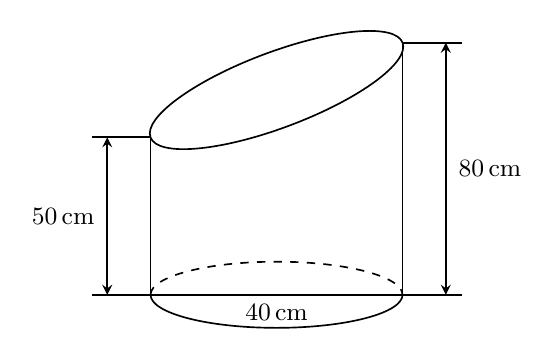
\begin{tikzpicture}[semithick, every node/.style={inner sep=1.5pt, font=\small}, >=stealth]
  % 下底椭圆：上半（背面）虚线，下半（正面）实线
  \draw[dashed] (-1.6,0) arc[start angle=180, end angle=0, x radius=1.6, y radius=0.42];
  \draw (-1.6,0) arc[start angle=180, end angle=360, x radius=1.6, y radius=0.42];
  % 底面直径
  \draw (-1.6,0) -- (1.6,0);
  \node at (0,-0.22) {$40\,\mathrm{cm}$};
  % 两条母线
  \draw (-1.6,0) -- (-1.6,2.0);
  \draw (1.6,0) -- (1.6,3.2);
  % 截口椭圆：两端点恰为两条母线的上端点 (-1.6,2.0) 与 (1.6,3.2)
  \draw[rotate around={20.6:(0,2.6)}] (0,2.6) ellipse (1.71 and 0.48);
  % 左侧 50 cm 标注
  \draw (-1.6,0) -- (-2.35,0);
  \draw (-1.6,2.0) -- (-2.35,2.0);
  \draw[<->] (-2.15,0) -- (-2.15,2.0);
  \node[left] at (-2.25,1.0) {$50\,\mathrm{cm}$};
  % 右侧 80 cm 标注
  \draw (1.6,0) -- (2.35,0);
  \draw (1.6,3.2) -- (2.35,3.2);
  \draw[<->] (2.15,0) -- (2.15,3.2);
  \node[right] at (2.25,1.6) {$80\,\mathrm{cm}$};
\end{tikzpicture}
\end{center}
\nopagebreak[4]
\end{question}
\endgroup
\begin{question}
\gkti{14}设 $n$ 阶方阵
\nopagebreak[4]
\[A_n=\begin{pmatrix}
1&3&5&\cdots&2n-1\\
2n+1&2n+3&2n+5&\cdots&4n-1\\
4n+1&4n+3&4n+5&\cdots&6n-1\\
\vdots&\vdots&\vdots&&\vdots\\
2n(n-1)+1&2n(n-1)+3&2n(n-1)+5&\cdots&2n^2-1
\end{pmatrix}.\]
任取 $A_n$ 中的一个元素，记为 $x_1$；划去 $x_1$ 所在的行和列，将剩下的元素按原来的位置关系组成 $n-1$ 阶方阵 $A_{n-1}$，任取 $A_{n-1}$ 中的一个元素，记为 $x_2$；划去 $x_2$ 所在的行和列，$\cdots\cdots$；将最后剩下的一个元素记为 $x_n$。记 $S_n=x_1+x_2+\cdots+x_n$，则 $\lim\limits_{n\to\infty}\dfrac{S_n}{n^3+1}=$ $\underline{\qquad}$。

\end{question}
\gkpart{二、选择题}

（本大题满分 $20$ 分）本大题共有 $4$ 题，每题有且只有一个正确答案。考生应在答题纸上的相应编号上，将代表答案的小方格涂黑，选对得 $5$ 分，否则一律得零分。

\begin{question}
\gkti{15}若空间三条直线 $a$、$b$、$c$ 满足 $a\perp b$，$b\perp c$，则直线 $a$ 与 $c$　[答]（　）

（A）一定平行。

（B）一定相交。

（C）一定是异面直线。

（D）平行、相交、是异面直线都有可能。

\end{question}
\begin{question}
\gkti{16}已知 $a_1$、$a_2\in(0,1)$。记 $M=a_1a_2$，$N=a_1+a_2-1$，则 $M$ 与 $N$ 的大小关系是　[答]（　）

（A）$M<N$。

（B）$M>N$。

（C）$M=N$。

（D）不确定。

\end{question}
\begin{question}
\gkti{17}已知抛物线 $C:y^2=x$ 与直线 $l:y=kx+1$。“$k\neq0$”是“直线 $l$ 与抛物线 $C$ 有两个不同的交点”的　[答]（　）

（A）充分不必要条件。

（B）必要不充分条件。

（C）充要条件。

（D）既不充分也不必要条件。

\end{question}
\begin{question}
\gkti{18}已知函数 $f(x)=\dfrac{1}{4-2^x}$ 的图像关于点 $P$ 对称，则点 $P$ 的坐标是　[答]（　）

（A）$\left(2,\dfrac12\right)$。

（B）$\left(2,\dfrac14\right)$。

（C）$\left(2,\dfrac18\right)$。

（D）$(0,0)$。

\end{question}
\gkpart{三、解答题}

（本大题满分 $74$ 分）本大题共有 $5$ 题，解答下列各题必须在答题纸相应编号的规定区域内写出必要的步骤。

\begin{question}
\gkti{19}\textbf{（本题满分 12 分）} 已知 $\tan\theta=a\ (a>1)$，求 $\dfrac{\sin\left(\dfrac\pi4+\theta\right)}{\sin\left(\dfrac\pi2-\theta\right)}\cdot\tan2\theta$ 的值。

\end{question}
\begin{question}
\gkti{20}\textbf{（本题满分 14 分）本题共有 2 个小题，第 1 小题满分 6 分，第 2 小题满分 8 分。} 已知函数 $f(x)=\log_a(8-2^x)$（$a>0$，且 $a\neq1$）。

（1）若函数 $f(x)$ 的反函数是其本身，求 $a$ 的值；

（2）当 $a>1$ 时，求函数 $y=f(x)+f(-x)$ 的最大值。

\Needspace{0.4\textheight}
\end{question}
\begingroup
\renewenvironment{question}{\Needspace{0.5\textheight}}{}
\begin{question}
\gkti{21}\textbf{（本题满分 14 分）本题共有 2 个小题，第 1 小题满分 6 分，第 2 小题满分 8 分。} 已知地球的半径约为 $6371$ 千米。上海的位置约为东经 $121^\circ$、北纬 $31^\circ$，大连的位置为东经 $121^\circ$、北纬 $39^\circ$，里斯本的位置约为西经 $10^\circ$、北纬 $39^\circ$。

（1）若飞机以平均速度 $720$ 千米/小时飞行，则从上海到大连的最短飞行时间约为多少小时（飞机飞行高度忽略不计，结果精确到 $0.1$ 小时）？

（2）求大连与里斯本之间的球面距离（结果精确到 $1$ 千米）。
\nopagebreak[4]
\begin{center}% 2010 年上海春季卷第 21 题：地球示意图（北极—南极、赤道、上海/大连所在经线与纬线、里斯本）。
% 来源 PDF：春季高考/2010/2010春季上海.pdf，SHA-256 24926e5272a6316cbaa399c0a097b3986ab34563db975016f98bae99f2274c56。
% 原页：第 2 页右栏中部（印刷页 2-38，《数学教学》2010 年第 2 期转载）。
% 重绘依据：球面轮廓 + 地轴虚线；北纬 39° 圈（实线）过大连、里斯本；
% 北纬 31° 圈（虚线）过上海；南侧另有赤道圈（实线）；经线用椭圆弧表示，
% 大连与上海同在东经 121° 经线上。
\begin{tikzpicture}[semithick, every node/.style={inner sep=1.5pt, font=\small}]
  % 球面轮廓与地轴
  \draw (0,0) circle (2);
  \draw[dashed] (0,2) -- (0,-2);
  % 纬圈：北纬 39°（实线，过大连、里斯本）
  \draw (0,1.15) ellipse (1.55 and 0.30);
  % 纬圈：北纬 31°（虚线，过上海）
  \draw[dashed] (0,0.66) ellipse (1.72 and 0.33);
  % 赤道（实线，位于视点下方）
  \draw (0,-0.45) ellipse (1.94 and 0.38);
  % 经线：左前方一条（实线）、过上海与大连一条（实线）、近中央背面一条（虚线）
  \draw (0,2) arc[start angle=90, end angle=270, x radius=0.55, y radius=2];
  \draw (0,2) arc[start angle=90, end angle=-90, x radius=0.735, y radius=2];
  \draw[dashed] (0,2) arc[start angle=90, end angle=-90, x radius=0.40, y radius=2];
  % 三地位置
  \fill (-1.55,1.15) circle (1.6pt);
  \node[left] at (-1.60,1.15) {里斯本};
  \fill (0.655,0.878) circle (1.6pt);
  \node at (0.60,1.15) {大连};
  \fill (0.727,0.361) circle (1.6pt);
  \node[right] at (0.755,0.361) {上海};
  % 球心与两极
  \node at (0.20,-0.10) {$O$};
  \node[above] at (0,2.05) {北极};
  \node[below] at (0,-2.05) {南极};
\end{tikzpicture}
\end{center}
\nopagebreak[4]
\end{question}
\endgroup
\begin{question}
\gkti{22}\textbf{（本题满分 16 分）本题共有 3 个小题，第 1 小题满分 4 分，第 2 小题满分 6 分，第 3 小题满分 6 分。} 在平面上，给定非零向量 $\vec b$。对任意向量 $\vec a$，定义 $\vec a'=\vec a-\dfrac{2\left(\vec a\cdot\vec b\right)}{\left|\vec b\right|^2}\vec b$。

（1）若 $\vec a=(2,3)$，$\vec b=(-1,3)$，求 $\vec a'$；

（2）若 $\vec b=(2,1)$，证明：若位置向量 $\vec a$ 的终点在直线 $Ax+By+C=0$ 上，则位置向量 $\vec a'$ 的终点也在一条直线上；

（3）已知存在单位向量 $\vec b$，当位置向量 $\vec a$ 的终点在抛物线 $C:x^2=y$ 上时，位置向量 $\vec a'$ 的终点总在抛物线 $C':y^2=x$ 上。曲线 $C$ 与 $C'$ 关于直线 $l$ 对称，问直线 $l$ 与向量 $\vec b$ 满足什么关系？

\end{question}
\begin{question}
\gkti{23}\textbf{（本题满分 18 分）本题共有 3 个小题，第 1 小题满分 4 分，第 2 小题满分 6 分，第 3 小题满分 8 分。} 已知首项为 $x_1$ 的数列 $\{x_n\}$ 满足 $x_{n+1}=\dfrac{ax_n}{x_n+1}$（$a$ 为常数）。

（1）若对任意的 $x_1\neq-1$，有 $x_{n+2}=x_n$ 对任意的 $n\in\mathbf N^*$ 都成立，求 $a$ 的值；

（2）当 $a=1$ 时，若 $x_1>0$，数列 $\{x_n\}$ 是递增数列还是递减数列？请说明理由；

（3）当 $a$ 确定后，数列 $\{x_n\}$ 由其首项 $x_1$ 确定。当 $a=2$ 时，通过对数列 $\{x_n\}$ 的探究，写出“$\{x_n\}$ 是有穷数列”的一个真命题（不必证明）。

说明：对于第（3）题，将根据写出真命题所体现的思维层次和对问题探究的完整性，给予不同的评分。

\end{question}